\documentclass{beamer}
\usetheme{Madrid}
\usecolortheme{default}

\usepackage{listings}
\lstset{
  language=Haskell,
  basicstyle=\ttfamily,
  keywordstyle=\color{blue},
  commentstyle=\color{green!40!black},
  stringstyle=\color{orange},
  showstringspaces=false,
  breaklines=true,
  frame=single,
  numbers=left,
  numberstyle=\tiny,
  numbersep=5pt,
  xleftmargin=10pt,
}

%Information to be included in the title page:
\title[Imperfect Forward Secrecy] %optional
{Imperfect Forward Secrecy: \newline How Diffie-Hellman Fails in Practice}
\subtitle{}
\author[Ines Cipullo] % (optional, for multiple authors)
{David Adrian, Karthikeyan Bhargavan, Zakir Durumeric, Pierrick Gaudry, Matthew Green,
J. Alex Halderman, Nadia Heninger, Drew Springall, Emmanuel Thomé, Luke Valenta,
Benjamin VanderSloot, Eric Wustrow, Santiago Zanella-Béguelink, Paul Zimmermann}
\institute[LCC - FCEIA] % (optional)
{
  Facultad de Ciencias Exactas, Ingeniería y Agrimensura,\\
  Universidad Nacional de Rosario.
}
\date[]{Ines Cipullo - Diciembre 2024}

\begin{document}

\frame{
    \titlepage
}

% Whitfield Diffie y Martin Hellman son quienes publican la idea original de la criptografía asimétrica
% Se investigo la seguridad del intercambio de claves Diffie-Hellman tal como se utiliza en los protocolos populares de Internet y se encontro que es menos seguro de lo que se cree comúnmente. La práctica común de utilizar parámetros estandarizados, predefinidos o ampliamente compartidos tiene el efecto de reducir drásticamente el costo de los ataques a gran escala, llevando algunos de ellos a ser factibles hoy en día, y las personas encargadas de poner en practica los protocolos no parecen enterados de esto

\begin{frame}
\frametitle{Protocolo Diffie-Hellman}
    \begin{itemize}
        \item<1-> Alice y Bob eligen un número primo $p$ y un generador $g$ %parametros publicos
        \item<1-> Alice $\rightarrow$ Bob: $A = g^a$ mod $p$
        \item<1-> Bob $\rightarrow$ Alice: $B = g^b$ mod $p$
        \item<1-> Alice y Bob calculan un \textbf{shared secret} a partir de $A$ y $B$: $g^{ab}$ mod $p$
        \item<1-> Este \textbf{shared secret} se utilizará como clave para el resto de la comunicación
    \end{itemize}
\end{frame}

\begin{frame}
\frametitle{Cómo vulnerar Diffie-Hellman?}
    Un atacante que observa el intercambio tiene acceso a $p$, $g$, $A$ y $B$.

    Para poder calcular la clave, su mejor opción es averiguar uno de los componentes privados, $a$ o $b$. Eso lo logra calculando el logaritmo discreto del valor público correspondiente: $A$ o $B$.

    % Se utiliza el algoritmo number field sieve para el calculo del logaritmo discreto. Este esta compuesto de 4 etapas: seleccion polinomial, sieving (o tamizado), algebra lineal y descenso. 
    % Notar como las 3 primeras etapas solo dependen del número primo p, que es público, y pueden ser precomputados (y reutilizado!). Finalmente, el ulitmo paso depende del resultado obtenido en la precomputacion y los valores de g e y, para obtener x. (y seria A o B, y x seria a o b)
    \begin{center}
        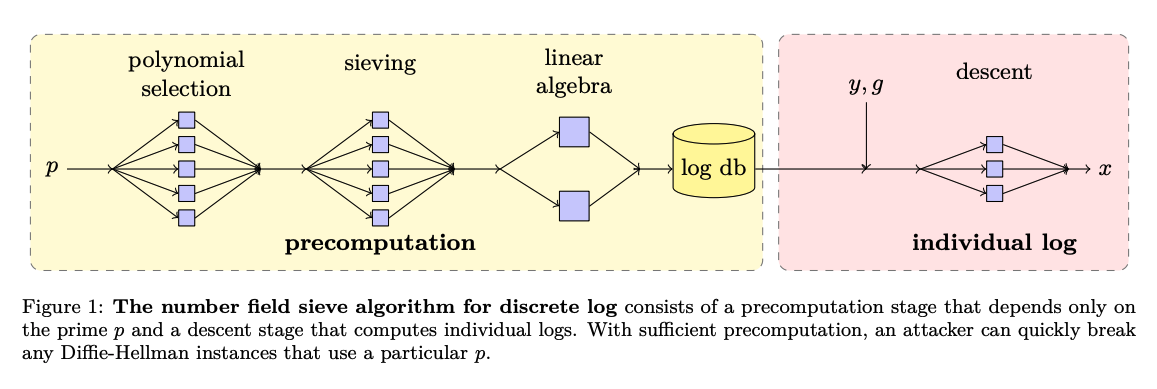
\includegraphics[scale=0.3]{figure1_dh.png}
    \end{center}
\end{frame}

\begin{frame}
    \frametitle{TLS y Diffie-Hellman}
    TLS es un protocolo criptográfico para comunicaciones entre aplicaciones, y su uso más usual es en HTTPS.
    
    TLS Handshake:
    \begin{itemize}
        \item<1-> El cliente envía al servidor un mensaje $ClientHello$ que incluye la lista de algoritmos criptográficos que soporta y un fresco $cr$
        \item<1-> El servidor elige un algoritmo y se lo comunica en un mensaje $ServerHello$, también incluyendo un fresco $sr$
    \end{itemize}

    % TLS soporta una gran variedad de métodos para negociar claves, entre ellos Diffie-Hellman, y $2/3$ de los sitios HTTPS permiten su uso. A su vez, 
    TLS soporta multiples variantes de Diffie-Hellman:
    \begin{itemize}
        \item<1-> Ephemeral Diffie-Hellman (DHE): es el definido originalmente y soporta números de cualquier cantidad de bits.
        \item<1-> Export-grade Diffie-Hellman (DHE\_Export): soporta números de un máximo de 512 bits, igual a DHE en el resto. La mayoría de clientes ya no lo aceptan.
    \end{itemize}
\end{frame}

\begin{frame}{Ataque LogJam}
    % El ataque LogJam es posible por una falla en la forma en la que TLS compone DHE y DHE_EXPORT. 
    % La idea es que el atacante se ubica entre cliente y servidor como un man-in-the-middle e intersecta los dos primeros mensajes donde se intenta acordar que algoritmo criptografico utilizar.
    % Todo esto es posible, ya que el siguiente mensaje firmado del servidor no incluye informacion sobre el algoritmo que fue elegido (es el mismo para DHE y DHE_EXPORT).

    \begin{center}
        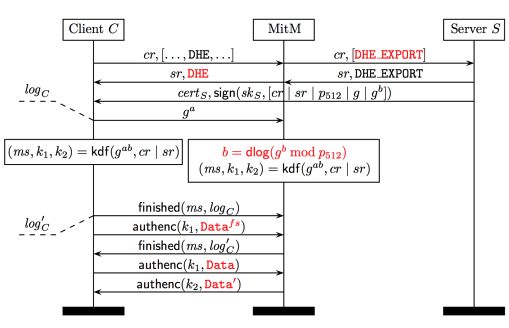
\includegraphics[scale=0.5]{figure2_dh.png}
    \end{center}
\end{frame}

\begin{frame}{Computaciones de logaritmo discreto}
    \begin{itemize}
        \item Se aplicó el algoritmo a 3 primos de 512 bits % (dos de los cuales comprenden el 92,3% de las conecciones que soportan DHE_EXPORT)
        \item Las precomputaciones tardaron 7 días por cada número primo
        \item Seleccion polinomial y sieving (o tamizado) se pueden paralelizar, el algebra lineal no tanto. Se decidio hacer más sieving, lo que permite que el paso de algerba lineal sea más corto, y que el paso de descenso sea más rápido.
        \item Se logra computar el último paso en un promedio de 70 segundos.
    \end{itemize}
\end{frame}

\begin{frame}{Reemplazar al servidor en la comunicación}
    Para poder completar el ataque, se debe poder computar el secreto en tiempo real, pero el algoritmo que se obtuvo tarda en promedio 70 segundos. Tecnicas para que el cliente espere nuestra respuesta:

    \begin{itemize}
        \item Si el usuario usa un \textbf{cliente de consola}, como git o curl, suelen tener un tiempo de espera mayor o no tener tiemout.
        \item \textbf{TLS warning alerts}: los navegadores ignoran estos mensajes pero se reinicia el contador del timeout, por lo que el atacante los puede utilizar para demorar el timeout.
        % Se logro demorar el timeout de Firefox indefinidamente, otros navegadores cierran la conexion luego de 1 min
        \item \textbf{Caching de claves efímeras}: algunos servidores no utilizan un valor fresco de $b$ para cada nueva conexión, sino que lo reutilizan para evitar tener que recalcular $g^b$. Si se obtiene la clave, se puede atacar futuras conexiones en tiempo real.
        % Esto se controla con opciones/parametros del protocolo, por lo que resalto la importancia de no utilizar los valores por defecto y revisar el impacto de los distintos parametros cuando se implemente
        \item \textbf{TLS false start}: algunos clientes envían datos sensibles antes de concluir el handshake para reducir la latencia de la comunicación, de esta forma el atacante luego puede desencriptarlo sin restricciones de tiempo.
    \end{itemize}
\end{frame}

\begin{frame}{Amenazas estatales}
    Como vimos, para poder llevar a cabo el ataque es necesario degradar la conexión para utilizar primos de 512 bits, ya que es lo que nos permite el poder de cómputo, y esto depende de la falla de TLS. 

    Qué pasaria si esto no fuese necesario?
    \begin{center}
        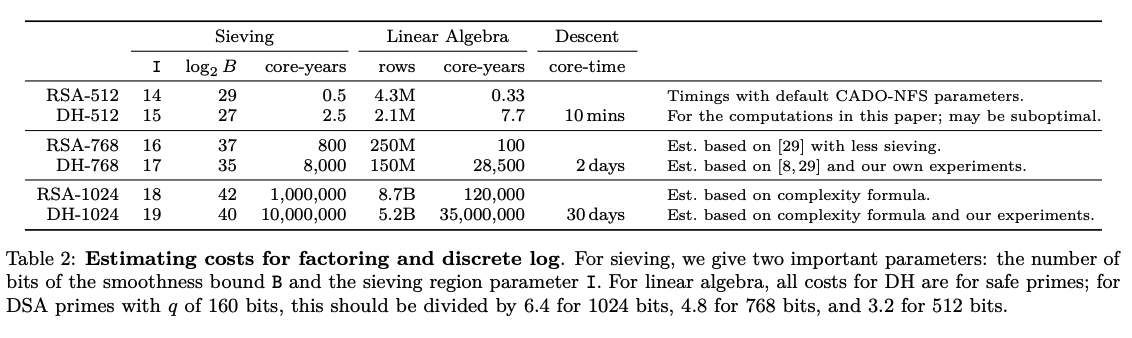
\includegraphics[scale=0.3]{figure3_dh.png}
    \end{center}
    % Extrapolando los resultados obtenidos en los experimentos, y junto con otros resultados computando algoritmos similares, se concluye que es posible computar el algoritmo de logaritmos discretos para numeros primos de 768 y 1024 con recursos de nivel estatal.
    % Si bien 45 millones de años nucleo parece demasiado, con presupuestos altos como son los de nivel estatal, se podria lograr optimizar y computar
\end{frame}

\begin{frame}{La NSA ya rompió DH 1024 bits?}
    Documentos clasificados que fueron publicados indicarían que sí.

    % Si bien no se describen las tecnicas utilizadas, proveen la arquitectura del sistema de ataque, que es la siguiente:

    \begin{center}
        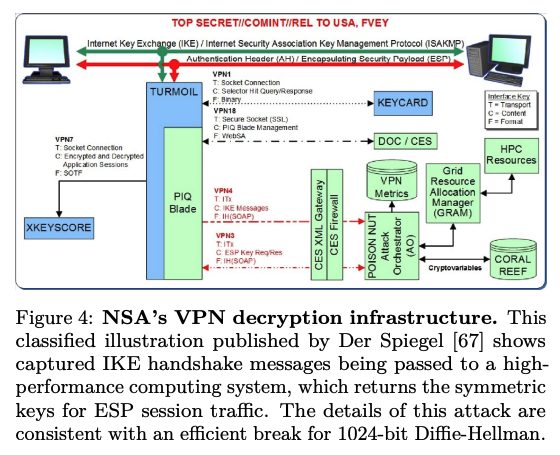
\includegraphics[scale=0.4]{figure4_dh.png}
    \end{center}

    % La NSA estaba atacando el protocolo IKE usado por VPNs para establecer claves de sesion, este protocolo utiliza Diffie-Hellman. Tambien se da alusion de que el ataque era producido escuchando pasivamente la red abierta (man-in-the-middle)
\end{frame}

\begin{frame}{Qué consecuencias tiene esto?}
    Asumiendo los recursos para poder precomputar una cantidad pequeña de grupos de 1024 bits, se analizó el uso de Diffie-Hellman en los protocolos más populares: IKE, HTTPS, SSH.

    % De todos los protocolos se toma un sample y se evalua si soportan los grupos oakley 1 y 2 (que son grupos muy populares de 768 bits y 1024 bits) y que grupo prefieren
    \textbf{IKE:}
    \begin{itemize}
        \item 31,8\% de IKEv1 soportan Oakley 1 (2,6\% lo prefiere)
        \item 86,1\% de IKEv1 soportan Oakley 2 (66,1\% lo prefiere)
        \item 19,7\% de IKEv2 soportan Oakley 1 (5,8\% lo prefiere)
        \item 91\% de IKEv2 soportan Oakley 2 (63,9\% lo prefiere)
    \end{itemize}

    \textbf{SSH:}
    \begin{itemize}
        \item 98.9\% soporta Oakley 2 (21\% lo prefiere)
    \end{itemize}\

    \textbf{HTTPS (sample: Alexa Top 1M):}
    \begin{itemize}
        \item 24\% de la conexiones utilizaron DH
        \item 84\% usa grupos de 1024 bits o menos (94\% usa 1 de los mismos 5 grupos)
    \end{itemize}
\end{frame}

\begin{frame}{Qué consecuencias tiene esto? (Cont.}
    TLS también se puede utilizar para asegurar comunicaciones entre servidores de email. Se evaluó un sample de todas las IPs publicas para IMAPS, POP3S y SMTP. % (protocolos que proveen servicios de email)
    
    \begin{itemize}
        \item Entre un 8\% y un 15\% soportan DHE\_EXPORT
        \item Alrededor del 75\% soporta DHE
    \end{itemize}
    
    Si se comprometieran los 10 primos de 1024 bits más usados por cada protocolo, se comprometerian las conexiones de más de 2M de servidores de mail.
\end{frame}

\begin{frame}{Alternativas de defensa}
    \begin{itemize}
        \item Utilizar Diffie-Hellman elíptico:
            \begin{itemize}
                \item Actualmente no se conocen ataques
                \item Es menos costoso computacionalmente para los usuarios
                % \item Hay cierto nivel de desconfianza porque lo publico la NSA
            \end{itemize}
        \item Incrementar el largo mínimo de las claves:
            \begin{itemize}
                \item 2048 bits como estándar
                \item No se debería aceptar menos de 1024 bits
            \end{itemize}
        \item Evitar utilizar los mismos grupos de primos:
            \begin{itemize}
                \item Evita que afecten las precomputaciones existentes
                \item No amortiza costos del atacante
            \end{itemize}
        \item No permitir debilitar deliberadamente protocolos criptográficos:
            \begin{itemize}
                \item DHE\_EXPORT se debería haber deprecado hace bastante
            \end{itemize}
    \end{itemize}
\end{frame}

% Conclusión: si bien Diffie-Hellman es parte de las bases de la criptografia, las formas en las que es implementado en la practica terminan debilitando la seguridad que deberia proveer el protocolo.

% References (needs a .bib file)
% \begin{frame}{Fuentes}
% \nocite{*}
% \bibliographystyle{plain}
% \bibliography{ref}
% \end{frame}

\end{document}